\documentclass[12pt,twoside, a4paper, twocolumn]{article}
\usepackage[utf8]{inputenc}
\usepackage[brazil]{babel}
\usepackage[margin = 0.5in]{geometry}
\usepackage{amsmath}
\usepackage{amsthm}
\usepackage{amssymb}
\usepackage{amsthm}
\usepackage{setspace}
\usepackage[americanvoltages,fulldiodes,siunitx]{circuitikz}
\usepackage{lipsum}
\usepackage{pgfplots}
\usepackage{ifthen}
\usepackage{adjustbox}
\usepackage[section]{placeins}
\usepackage{hyperref}
\usepackage{graphicx}
\usepackage{amsmath}
\usepackage{amsthm}
\usepackage{amssymb}
\usepackage{amsthm}
\usepackage{setspace}
\usepackage[americanvoltages,fulldiodes,siunitx]{circuitikz}
\usepackage{lipsum}
\usepackage{pgfplots}
\usepackage{ifthen}
\usepackage{adjustbox}
\usepackage[section]{placeins}
\usepackage{hyperref}
\usepackage{graphicx}
\usepackage{adjustbox}
\usepackage{indentfirst}

\pgfplotsset{compat=newest}
\graphicspath{ {./images/} }
%  #1 color - optional #2 x_0 #3 y_0 #4 x_f #5 y_f #6 name - optional  #7 true if adding lines to axis
\newcommand{\drawvector} [9] [color=cyan] {
\draw[line width=1.5pt,#1,-stealth](axis cs: #2, #3)--(axis cs: #4, #5) node[anchor=south west]{$#6$};
\ifthenelse{\equal{#7}{true}}{
\draw[line width=1pt,#1, dashed](axis cs: #4, #5)--(axis cs: #4, 0) node[anchor= north west]{$#8$};
\draw[line width=1pt,#1, dashed](axis cs: #4, #5)--(axis cs: 0, #5) node[anchor=south east]{$#9$};
}
{}
}
\newcommand\deriv[2]{\frac{\mathrm d #1}{\mathrm d #2}}
\title{Estudo dirigido sobre Amplificadores Operacionais}
\author{Henrique da Silva \\ henrique.pedro@ufpe.br}
\date{\today}
\pgfplotsset{width = 10cm, compat = 1.9}
\begin{document}
\maketitle
\pagenumbering{gobble}
\newpage
%pagenumbering{roman}
\tableofcontents
\newpage

\section{Introdução}


Neste relatório, vamos discutir amplificadores operacionais, e algumas configurações úteis de circuitos que utilizam amp ops.


Todos arquivos utilizados para criar este relatório, e o relatorio em si estão em:  \url{https://github.com/Shapis/ufpe_ee/tree/main/6th semester}


\section{Amplificadores Operacionais}


Os amplificadores operacionais (Amps Op) são dispositivos eletrônicos que amplificam um sinal de entrada diferencial. Eles são amplamente utilizados em circuitos eletrônicos devido às suas excelentes características de amplificação, alta impedância de entrada e baixa impedância de saída.


Os amplificadores operacionais possuem diversas características e propriedades que os tornam componentes essenciais em projetos eletrônicos. Vamos explorar algumas das características mais importantes.


\subsection{Ganho de Tensão de Malha Aberta}


O ganho de tensão de malha aberta é uma das características fundamentais dos amplificadores operacionais. Representado por Aol, esse parâmetro indica a magnitude do ganho de tensão quando não há realimentação externa no amplificador. Idealmente, um amplificador operacional ideal possui um ganho de tensão de malha aberta infinita. No entanto, na prática, esse valor é bastante elevado, geralmente da ordem de $10^5$ a $10^6$.


\subsection{Impedância de Entrada}


A impedância de entrada de um amplificador operacional é uma medida da resistência que ele apresenta aos sinais de entrada. Idealmente, um amplificador operacional tem uma impedância de entrada infinita, o que significa que não há corrente de entrada fluindo para o amplificador, resultando em uma carga desprezível para a fonte de sinal. Essa alta impedância de entrada garante que o amplificador não influencie significativamente o circuito de entrada.


\subsection{Impedância de Saída}


A impedância de saída é a resistência que o amplificador operacional apresenta ao circuito externo conectado à sua saída. Idealmente, um amplificador operacional tem uma impedância de saída zero, o que significa que ele pode fornecer corrente de saída sem restrições e sem queda de tensão significativa. No entanto, na prática, a impedância de saída é baixa, mas não exatamente zero.


\subsection{CMRR (Rejeição de Modo Comum)}


A rejeição de modo comum é uma medida da capacidade do amplificador operacional de rejeitar sinais de entrada que são comuns a ambas as entradas (modo comum), como ruídos indesejados ou interferências. O CMRR é expresso em decibéis (dB) e representa a relação entre o ganho diferencial (ganho para sinais de entrada diferenciais) e o ganho de modo comum (ganho para sinais de entrada comuns).


\subsection{Resposta em Frequência}


A resposta em frequência de um amplificador operacional indica como o ganho do amplificador varia em função da frequência do sinal de entrada. Idealmente, um amplificador operacional possui uma resposta em frequência plana, ou seja, mantém um ganho constante em uma faixa ampla de frequências. No entanto, na prática, a resposta em frequência pode ser limitada por fatores como capacitâncias internas, eletroquímica dos componentes e características do projeto.


\subsection{Largura de Banda}


A largura de banda é a faixa de frequência na qual o amplificador operacional possui um ganho de tensão de malha aberta dentro de um limite especificado. É comum definir a largura de banda como a frequência na qual o ganho de tensão de malha aberta cai em 3 dB em relação ao seu valor máximo. É importante considerar a largura de banda ao projetar circuitos com amplificadores operacionais para garantir que a resposta em frequência seja adequada às necessidades do sistema.


\subsection{Taxa de Subida}


A taxa de subida é uma medida da velocidade com que o amplificador operacional pode responder a mudanças rápidas nos sinais de entrada. É expressa em volts por microssegundo (V/µs) e representa a variação máxima permitida na tensão de saída por unidade de tempo. A taxa de subida está relacionada à capacidade do amplificador operacional de acompanhar sinais de entrada de alta frequência.


\subsection{Corrente de Bias}


A corrente de bias é a corrente contínua necessária para operar o amplificador operacional. É a corrente que flui pelas entradas do amplificador quando não há sinal de entrada aplicado. A corrente de bias pode afetar o consumo de energia e a estabilidade do amplificador operacional.


\section{Amplificador Operacional Ideal}


O Amplificador Operacional Ideal é um modelo teórico usado como referência para entender o comportamento dos amplificadores operacionais na teoria. Embora os amplificadores operacionais reais não possam atingir todas as características ideais, o modelo ideal é útil para análises e projetos de circuitos, fornecendo uma base para compreender as funcionalidades desejáveis do amplificador.


\subsection{Ganho de Tensão Infinito}


No modelo ideal, o amplificador operacional possui um ganho de tensão de malha aberta infinita. Isso significa que qualquer diferença de tensão aplicada às entradas do amplificador resultará em uma tensão de saída infinitamente amplificada. O ganho de tensão infinito é uma característica desejável, pois permite que o amplificador amplifique com precisão os sinais de entrada.


\subsection{Impedância de Entrada Infinita}


O amplificador operacional ideal possui uma impedância de entrada infinita, o que significa que nenhum fluxo de corrente ocorre nas entradas do amplificador. Isso é desejável porque evita a carga do sinal de entrada, garantindo que o amplificador não afete significativamente o circuito de entrada.


\subsection{Impedância de Saída Nula}


O amplificador operacional ideal possui uma impedância de saída nula, o que significa que pode fornecer corrente de saída sem restrições e sem queda de tensão significativa. Essa característica permite a conexão eficiente de cargas externas ao amplificador sem causar distorção ou perda de sinal.


\subsection{Resposta em Frequência Infinita}


O amplificador operacional ideal tem uma resposta em frequência infinita, o que significa que pode amplificar sinais em uma faixa de frequência ilimitada. Isso permite a amplificação precisa de sinais de alta frequência sem atenuação ou distorção significativa. No entanto, na prática, os amplificadores operacionais reais têm uma largura de banda limitada devido a limitações físicas.


\subsection{Rejeição de Modo Comum Infinita}


O amplificador operacional ideal possui uma rejeição de modo comum infinita, o que significa que ele é capaz de rejeitar completamente sinais de entrada comuns a ambas as entradas (ruído comum). Isso resulta em uma amplificação precisa apenas dos sinais diferenciais desejados, eliminando interferências indesejadas.


\subsection{Taxa de Subida Infinita}


No modelo ideal, o amplificador operacional tem uma taxa de subida infinita, o que significa que é capaz de responder instantaneamente a mudanças rápidas nos sinais de entrada. Essa característica é essencial para amplificar sinais de alta frequência e variações rápidas sem distorção.


\subsection{Alimentação Simétrica}


O amplificador operacional ideal é alimentado com uma fonte de alimentação simétrica, o que significa que as tensões de alimentação positiva e negativa são iguais em magnitude e opostas em polaridade. Isso permite que o amplificador opere em uma faixa de tensão simétrica em relação ao terra, facilitando o projeto e a operação de circuitos.


\subsection{Limitações do Modelo Ideal}


É importante ressaltar que o modelo ideal do amplificador operacional não reflete as características dos amplificadores operacionais reais. Amplificadores operacionais reais possuem limitações, como ganho finito, impedância de entrada não infinita, impedância de saída não nula, resposta em frequência limitada, rejeição de modo comum limitada e slew rate finito. Portanto, ao projetar circuitos com amplificadores operacionais reais, é necessário levar em consideração essas limitações e selecionar amplificadores que atendam aos requisitos específicos da aplicação.


Embora o amplificador operacional ideal seja um modelo teórico, sua utilização é valiosa para analisar circuitos e entender os princípios básicos de funcionamento dos amplificadores operacionais. A partir dessa base teórica, podem ser desenvolvidos modelos mais realistas para simular e projetar circuitos que levem em conta as características dos amplificadores operacionais reais.




\newpage


\section{Amplificador Inversor}


O amplificador inversor é um dos circuitos mais comuns e básicos que utiliza um amplificador operacional. Ele amplifica um sinal de entrada diferencialmente, produzindo um sinal de saída que é uma versão invertida em relação ao sinal de entrada. O amplificador inversor é amplamente utilizado em aplicações de amplificação de sinais, ganho de tensão e processamento de sinais.




\subsection{O Circuito}




\begin{figure}[h]
    \centering
    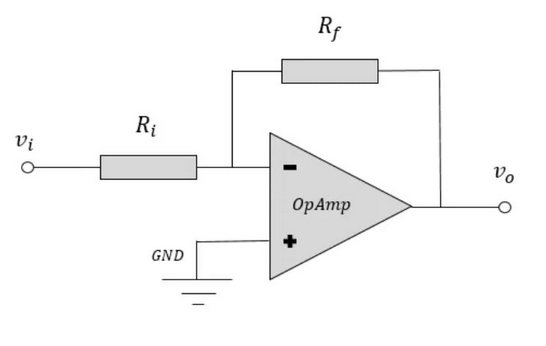
\includegraphics[width=1\columnwidth]{images/opamp_inversor.png}
    \caption{Amplificador operacional em configuração inversora.}
\end{figure}




\subsection{Princípio de Funcionamento}






O circuito do amplificador inversor consiste em um amplificador operacional e dois resistores: um resistor de entrada $R_i$ conectado à entrada do amplificador e um resistor de realimentação $R_f$ conectado entre a saída do amplificador e a entrada inversora. O sinal de entrada é aplicado ao terminal não inversor do amplificador operacional, enquanto a saída é medida no terminal inversor.


O amplificador operacional ideal possui uma impedância de entrada infinita, o que significa que nenhuma corrente flui para a entrada. Assumindo isso, a corrente que flui através do resistor de realimentação é igual à corrente que flui através do resistor de entrada. Isso ocorre porque não há caminho para a corrente entrar no terminal inversor do amplificador operacional.


Usando a lei de Ohm, podemos determinar a relação entre o sinal de entrada $V_i$, o resistor de entrada $R_i$, o sinal de saída $V_o$ e o resistor de realimentação $R_f$. A tensão na entrada inversora do amplificador operacional é virtualmente igual à tensão na entrada não inversora devido às altas impedâncias envolvidas. Portanto, podemos escrever a seguinte equação:


\begin{equation}
    V_i = R_i I_i
\end{equation}


onde $I_i$ é a corrente que flui através do resistor de entrada. Essa corrente também é igual à corrente que flui através do resistor de realimentação, uma vez que não há corrente que entra no terminal inversor do amplificador operacional ideal. Portanto, podemos escrever:


\begin{equation}
    I_i = \frac{V_o - V_i}{R_f}
\end{equation}


Substituindo a equação (2) na equação (1), obtemos:


\begin{equation}
    V_i = R_i I_i \frac{V_o - V_i}{R_f}
\end{equation}


Reorganizando a equação, encontramos a relação entre o sinal de saída e o sinal de entrada:


\begin{equation}
    V_o = - \frac{R_f}{R_i} V_i
\end{equation}


Essa equação indica que o amplificador inversor produz uma saída que é uma versão amplificada e invertida do sinal de entrada. O fator de amplificação é determinado pela relação entre os resistores de realimentação e de entrada (Rf/Rin). O sinal de saída é polarizado de maneira oposta ao sinal de entrada.


\subsection{Aplicações do Amplificador Inversor}


O amplificador inversor é amplamente utilizado em várias aplicações devido à sua capacidade de amplificar sinais e fornecer ganho de tensão. Algumas das principais aplicações incluem:


\begin{itemize}
    \item Amplificação de Sinais: O amplificador inversor é usado para amplificar sinais de baixa amplitude, proporcionando ganho de tensão. Isso é útil em aplicações de áudio, instrumentação, comunicações e muitos outros sistemas em que os sinais precisam ser amplificados para posterior processamento ou transmissão.
    \item Conversão de Impedância: O amplificador inversor pode ser usado para converter a impedância de entrada de um circuito, permitindo a interface entre diferentes dispositivos ou estágios de amplificação. Isso é especialmente útil quando a impedância de saída de uma fonte de sinal não é compatível com a impedância de entrada do próximo estágio do circuito.
    \item Atenuação de Sinais: O amplificador inversor também pode ser usado para atenuar sinais. Isso é alcançado selecionando a relação adequada entre os resistores de realimentação e de entrada, resultando em um fator de amplificação menor que 1.
    \item Circuitos de Controle: O amplificador inversor é usado em circuitos de controle e realimentação, onde o sinal de saída é comparado com um sinal de referência para ajustar e estabilizar sistemas. Essa configuração é amplamente utilizada em amplificadores de potência, sistemas de controle de temperatura, sistemas de controle de velocidade e muito mais.
    \item Circuitos de Filtro: O amplificador inversor pode ser usado em circuitos de filtro ativo para amplificar e filtrar sinais em determinadas faixas de frequência. A combinação de componentes passivos, como resistores e capacitores, com o amplificador inversor permite a criação de filtros de alta qualidade e precisão.
\end{itemize}


Essas são apenas algumas das aplicações do amplificador inversor. Sua simplicidade, versatilidade e capacidade de fornecer ganho de tensão tornam-no um componente fundamental em muitos circuitos e sistemas eletrônicos.


\newpage
\section{Amplificador Não Inversor}


O amplificador não inversor é outro circuito comumente utilizado que utiliza um amplificador operacional para amplificar um sinal de entrada. Ao contrário do amplificador inversor, o amplificador não inversor produz uma saída que tem a mesma polaridade que o sinal de entrada. Ele fornece ganho de tensão positivo e é amplamente utilizado em aplicações que requerem amplificação precisa e não requerem inversão de fase do sinal.


\subsection{O Circuito}


\begin{figure}[h]
    \centering
    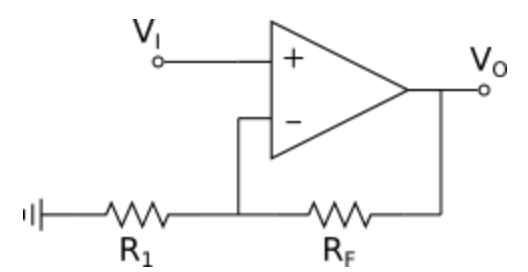
\includegraphics[width=1\columnwidth]{images/opamp_naoinversor.png}
    \caption{Amplificador operacional em configuração não inversora.}
\end{figure}


\subsection{Princípio de Funcionamento}


O circuito do amplificador não inversor também consiste em um amplificador operacional e dois resistores: um resistor de entrada $R_1$ conectado entre a saída inversora e o terra, e um resistor de realimentação $R_f$ conectado entre a saída do amplificador e a entrada inversora. O sinal de entrada é aplicado ao terminal não inversor do amplificador operacional, enquanto a saída é medida no $V_o$.


Assumindo que o amplificador operacional ideal possui uma impedância de entrada infinita, a corrente que flui através do resistor de realimentação é igual à corrente que flui através do resistor $R_1$. Como a corrente não flui para o terminal inversor do amplificador operacional.


Aplicando a lei de Ohm, podemos determinar a relação entre o sinal de entrada $V_i$, o resistor $R_1$, o sinal de saída $V_o$ e o resistor de realimentação $R_f$. A tensão na entrada não inversora do amplificador operacional é virtualmente igual à tensão na entrada inversora, devido às altas impedâncias envolvidas. Portanto, podemos escrever a seguinte equação:


\begin{equation}
    V_i = V_n = V_p,
\end{equation}


onde $V_p$ é a tensão na entrada não inversora e $V_n$ é a tensão na entrada inversora.


Considerando a relação de corrente entre o resistor $R_1$ e o resistor de realimentação $R_f$, temos:


\begin{equation}
    \frac{V_i}{R_1} = I_1 = I_o
\end{equation}


onde $I_i$ é a corrente que flui através do resistor $R_1$ e $I_o$ é a corrente que flui através do resistor de realimentação.


Aplicando a lei de Ohm novamente, podemos escrever a seguinte equação:


\begin{equation}
    V_o = V_n + R_f I_1 = V_i + R_f I_1 = V_1 (1 + \frac{R_f}{R_1})
\end{equation}


Assim obtemos o seguinte ganho:


\begin{equation}
    G_o = \frac{V_o}{V_i} = 1 + \frac{R_f}{R_1}
\end{equation}


Essa equação indica que o amplificador não inversor produz uma saída que é uma versão amplificada e não invertida do sinal de entrada. O fator de amplificação é determinado pela relação entre os resistores de realimentação e de entrada $1 + \frac{R_f}{R_1}$. O sinal de saída é polarizado da mesma maneira que o sinal de entrada.


\subsection{Aplicações do Amplificador Não Inversor}


O amplificador não inversor é amplamente utilizado em várias aplicações que requerem amplificação de sinal e ganho de tensão sem inversão de polaridade. Algumas das principais aplicações incluem:


\begin{itemize}
    \item Amplificação de Sinais: O amplificador não inversor é usado para amplificar sinais de baixa amplitude, fornecendo um ganho de tensão positivo. Isso é útil em aplicações onde um sinal precisa ser amplificado sem alterar sua polaridade.
    \item Buffer de Sinal: O amplificador não inversor também é usado como um buffer de sinal para isolar circuitos de alta impedância de circuitos de baixa impedância. Ele evita a carga do sinal de entrada e fornece uma fonte de baixa impedância para alimentar outros dispositivos ou estágios de amplificação.
    \item Amplificador de Instrumentação: O amplificador não inversor é comumente usado em aplicações de amplificação de instrumentação, onde a precisão e a fidelidade do sinal são essenciais. Ele é usado para amplificar e isolar sinais de sensores, como termopares, pontes de Wheatstone e sensores de pressão, antes de serem processados por outros circuitos.
    \item Amplificação de Áudio: O amplificador não inversor é usado em amplificadores de áudio para amplificar o sinal de entrada de uma fonte de áudio, como um tocador de música ou um microfone. Ele fornece um ganho de tensão positivo e garante uma reprodução fiel do sinal de áudio sem inversão de fase.
    \item Circuitos de Controle: O amplificador não inversor é usado em circuitos de controle onde um sinal de referência é comparado com o sinal de saída para ajustar e estabilizar sistemas. Ele é usado em controladores PID (Proporcional-Integral-Derivativo), sistemas de controle de temperatura, sistemas de controle de velocidade e muito mais.
\end{itemize}


O amplificador não inversor é um componente versátil e amplamente utilizado em muitas aplicações eletrônicas. Sua capacidade de fornecer ganho de tensão sem inversão de polaridade o torna uma escolha popular em projetos que exigem amplificação de sinal e processamento de sinal preciso.


\newpage


\section{Amplificador Somador}


O amplificador somador, também conhecido como amplificador operacional somador, é um circuito que permite combinar múltiplos sinais de entrada em um único sinal de saída. Ele realiza a função matemática de somar as tensões de entrada ponderadas por coeficientes de ponderação definidos pelos resistores utilizados no circuito. O amplificador somador é amplamente utilizado em aplicações onde é necessário combinar sinais de diferentes fontes e realizar operações de soma ou subtração ponderada.


\subsection{O Circuito}


\begin{figure}[h]
    \centering
    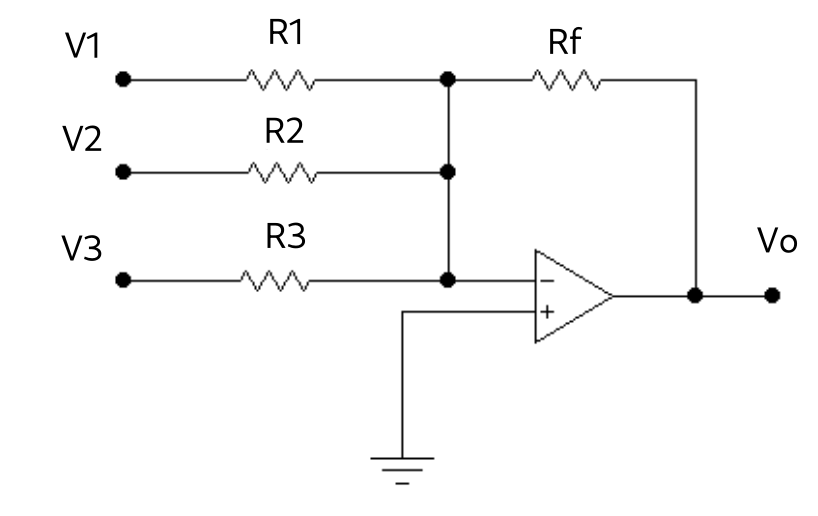
\includegraphics[width=1\columnwidth]{images/opamp_somador.png}
    \caption{Amplificador operacional em configuração somadora.}
\end{figure}


\subsection{Princípio de Funcionamento}


O circuito do amplificador somador é composto por um amplificador operacional e vários resistores. Cada sinal de entrada é conectado a um resistor individual, e todas as junções dos resistores são conectadas ao terminal inversor do amplificador operacional. O terminal não inversor é conectado ao terra.


O princípio de funcionamento do amplificador somador é baseado na propriedade do amplificador operacional ideal de ter uma impedância de entrada infinita. Isso significa que nenhum sinal de corrente flui para o terminal inversor, e, portanto, todas as correntes de entrada fluem apenas através dos resistores conectados às entradas.


A corrente de entrada em cada resistor é determinada pela lei de Ohm e é proporcional à tensão de entrada dividida pela resistência correspondente. Portanto, a corrente total que flui para o terminal inversor do amplificador operacional é a soma das correntes individuais ponderadas. Isso resulta em uma tensão de saída que é a soma das tensões de entrada ponderadas.


Por exemplo, considerando um amplificador somador com três entradas $V_1$, $V_2$ e $V_3$ e três resistores $R_1$, $R_2$ e $R_3$, a corrente total que flui para o terminal inversor é dada por:


\begin{equation}
    I_i = \frac{V_1}{R_1} + \frac{V_2}{R_2} + \frac{V_3}{R_3}
\end{equation}


Essa corrente também é igual à corrente que flui através do resistor de realimentação $R_f$, uma vez que não há corrente que entra no terminal inversor do amplificador operacional ideal. Portanto, podemos escrever:


\begin{equation}
    I_i = \frac{V_{out} - V_n}{R_f}
\end{equation}


onde $V_n$ é a tensão no terminal inversor do amplificador operacional, que é virtualmente igual a zero devido ao terra virtual.


Ao igualar as duas equações acima, podemos determinar a relação entre as tensões de entrada e a tensão de saída:


\begin{equation}
    V_{out} = - \frac{R_f}{R_1} V_1 - \frac{R_f}{R_2} V_2 - \frac{R_f}{R_3} V_3
\end{equation}


Essa equação mostra que o amplificador somador produz uma saída que é a soma ponderada das tensões de entrada. Os coeficientes de ponderação são determinados pela relação entre os resistores de realimentação e os resistores de entrada.


\subsection{Aplicações do Amplificador Somador}


O amplificador somador é amplamente utilizado em diversas aplicações onde é necessário combinar sinais de diferentes fontes e realizar operações de soma ou subtração ponderada. Algumas das principais aplicações incluem:


\begin{itemize}
    \item Conversores Analógico-Digital (ADC): O amplificador somador é utilizado em estágios de conversão analógico-digital para combinar os sinais analógicos de entrada e convertê-los em uma representação digital. Cada sinal de entrada é ponderado e somado para obter o valor digital correspondente.
    \item Misturadores de Áudio: Em sistemas de mixagem de áudio, o amplificador somador é usado para combinar os sinais de diferentes fontes, como microfones e instrumentos musicais. Os sinais são ponderados e somados para criar a mixagem final.
    \item Processamento de Sinais: O amplificador somador é usado em várias aplicações de processamento de sinais, como filtragem adaptativa, equalização de áudio e correção de distorção. Os sinais de entrada são combinados e processados de acordo com os pesos definidos pelos resistores.
    \item Controle Automático: O amplificador somador é utilizado em sistemas de controle automático, como controle de temperatura, controle de velocidade e controle de posição. Os sinais de entrada, que representam os valores de referência e as variáveis de controle, são combinados e comparados para ajustar e estabilizar o sistema.
\end{itemize}


O amplificador somador é um componente versátil que permite combinar sinais de entrada e realizar operações matemáticas ponderadas. Sua utilização é ampla em sistemas eletrônicos que requerem a combinação e processamento de múltiplos sinais.


\newpage


\section{Amplificador Diferencial}


O amplificador diferencial é um circuito que amplifica a diferença de potencial entre duas entradas, enquanto rejeita sinais comuns presentes em ambas as entradas. É uma configuração comum de amplificador operacional que é amplamente utilizado em aplicações onde é necessário amplificar e processar sinais diferenciais, como na amplificação de sinais de sensores, na transmissão de dados diferenciais e na filtragem de ruído comum.


\subsection{O Circuito}


\begin{figure}[h]
    \centering
    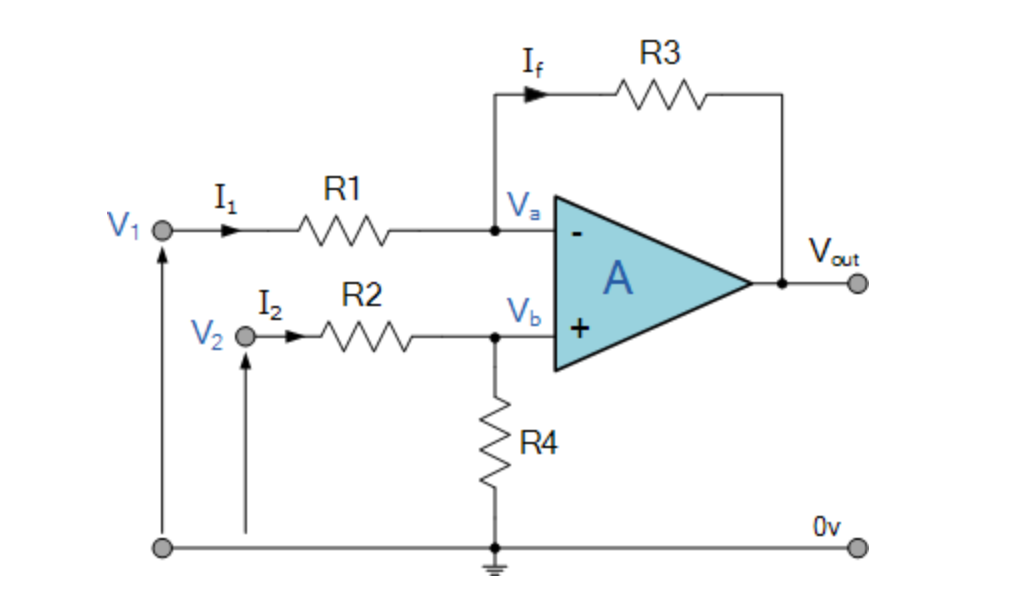
\includegraphics[width=1\columnwidth]{images/opamp_diferencial.png}
    \caption{Amplificador operacional em configuração diferencial.}
\end{figure}


\subsection{Princípio de Funcionamento}


O circuito do amplificador operacional diferencial consiste em dois estágios: o estágio de entrada diferencial e o estágio de saída. No estágio de entrada, dois resistores são conectados às entradas inversoras e não inversora do amplificador operacional. A saída é obtida no estágio seguinte, que é configurado como um amplificador inversor.


Quando um sinal diferencial é aplicado às entradas do amplificador operacional, a diferença de tensão é amplificada pelo ganho do amplificador operacional. Esse ganho é determinado pelos resistores de realimentação do estágio de saída. A saída do amplificador é dada pela diferença de potencial amplificada entre as entradas, multiplicada pelo ganho do estágio de saída.


Ao mesmo tempo, qualquer sinal comum presente nas duas entradas é rejeitado pelo amplificador operacional diferencial. Isso ocorre porque o amplificador operacional é projetado para amplificar apenas a diferença de tensão entre suas entradas e rejeitar o sinal comum. Essa rejeição é devido à maneira como o circuito está configurado, com as entradas inversora e não inversora conectadas por meio de resistores de igual valor.


Essa configuração resulta em uma relação de ganho diferencial alta e uma relação de ganho comum baixa. Portanto, a amplificação diferencial é alta para o sinal de entrada diferencial, enquanto o sinal comum é atenuado na saída.


\subsection{Equações}


Resolverei o sistema por superposição. Inicialmente fazendo $V_1 = 0$ e após $V_2 = 0$. E a nossa saída será a soma das saídas dos dois casos.


\begin{equation}
    \begin{aligned}
        I_1 = \frac{V_1 - V_a}{R_1} \\
        I_2 = \frac{V_2 - V_b}{R_2} \\
        I_3 = \frac{V_a - V_o}{R_3} \\
    \end{aligned}
\end{equation}


Temos o terra virtual que nos dá:


\begin{equation}
    V_a = V_b
\end{equation}


E por divisor de tensão temos:


\begin{equation}
    V_b = V_2 \frac{R_4}{R_2 + R_4}
\end{equation}


Agora fazendo $V_1 = 0$ primeiro e depois $V_2 = 0$ temos:


\begin{equation}
    \begin{aligned}
         & V_{out(a)} = -V_1 \frac{R_3}{R_1}                                                          \\
         & V_{out(b)} = V_2 \left( \frac{R_4}{R_2 + R_4} \right) \left( \frac{R_1 + R_3}{R_1} \right)
    \end{aligned}
\end{equation}


E a nossa saída combinada será $V_o = V_{out(a)} + V_{out(b)}$:


\begin{equation}
    V_o = -V_1 \frac{R_3}{R_1} + V_2 \left( \frac{R_4}{R_2 + R_4} \right) \left( \frac{R_1 + R_3}{R_1} \right)
\end{equation}


Que simplificando chegamos a equação que rege a saída do nosso amplificador diferencial:


\begin{equation}
    V_o = \frac{R_3}{R_1} \left( V_2 - V_1 \right)
\end{equation}


\section{Aplicações do Amplificador Operacional Diferencial}


O amplificador operacional diferencial tem diversas aplicações em eletrônica e sistemas de medição. Algumas das principais aplicações incluem:


\begin{itemize}
    \item Amplificação de Sinais de Sensores: O amplificador operacional diferencial é amplamente utilizado para amplificar sinais de sensores diferenciais, como termopares, células de carga e pontes de Wheatstone. Ele permite a amplificação precisa da diferença de tensão gerada pelos sensores, enquanto rejeita os ruídos comuns.
    \item Filtro de Rejeição de Ruído Comum: O amplificador operacional diferencial é utilizado em circuitos de filtragem para rejeitar o ruído comum presente em ambos os sinais de entrada. Isso é particularmente útil em aplicações onde a redução do ruído é crucial, como em sistemas de áudio de alta fidelidade.
    \item Amplificação de Sinais de Baixa Amplitude: O amplificador operacional diferencial é usado para amplificar sinais de baixa amplitude, como sinais de sensores sensíveis ou sinais de áudio fracos. Ele permite uma amplificação precisa e de baixo ruído, proporcionando uma melhor relação sinal-ruído.
    \item Comparadores de Tensão: O amplificador operacional diferencial também pode ser usado como um comparador de tensão, onde a diferença de tensão entre as entradas é comparada com um valor de referência. Isso é comumente utilizado em circuitos de detecção de níveis ou em sistemas de controle onde é necessário tomar decisões com base em comparações de tensão.
\end{itemize}


O amplificador operacional diferencial é um circuito versátil que permite amplificar sinais diferenciais enquanto rejeita sinais comuns indesejados. Sua configuração simples e suas propriedades de amplificação e rejeição tornam-no uma escolha popular em muitas aplicações de eletrônica e sistemas de medição.


\newpage


\section{Amplificadores Operacionais em Cascata}


Os circuitos com amplificadores operacionais em cascata são configurações nas quais dois ou mais amplificadores operacionais são conectados em série para alcançar um desempenho amplificado mais sofisticado e complexo. Essa técnica é amplamente utilizada em aplicações de eletrônica, onde é necessário amplificar sinais com maior ganho, melhor resposta em frequência, maior precisão ou realizar operações matemáticas complexas.


Ao conectar amplificadores operacionais em cascata, os sinais de entrada passam por vários estágios de amplificação, onde cada amplificador contribui para o ganho total e outras características do circuito. Isso permite a criação de circuitos mais poderosos e flexíveis, adaptados às necessidades específicas de cada aplicação.


\subsection{Benefícios dos Circuitos em Cascata}


Os circuitos com amplificadores operacionais em cascata apresentam diversos benefícios em relação a circuitos de amplificação simples. Alguns desses benefícios incluem:


\begin{itemize}
    \item Ganho Total Aumentado: Ao conectar amplificadores em cascata, o ganho total do circuito é multiplicado pelo ganho de cada estágio individual. Isso permite amplificar sinais com maior magnitude, tornando os circuitos em cascata adequados para aplicações de amplificação de sinais fracos.
    \item Resposta em Frequência Aprimorada: Cada estágio de amplificação em cascata contribui para a resposta em frequência global do circuito. Ao utilizar amplificadores com características de resposta em frequência complementares, é possível estender a faixa de frequência efetiva do circuito.
    \item Maior Impedância de Entrada: Os circuitos em cascata podem ser projetados de forma a apresentar uma impedância de entrada total maior em comparação com um único amplificador. Isso é útil em aplicações em que é necessário minimizar a carga sobre a fonte de sinal e preservar a integridade do sinal de entrada.
    \item Operações Matemáticas Complexas: Os circuitos em cascata também podem ser projetados para realizar operações matemáticas complexas, como multiplicação, divisão, integração e diferenciação. Isso é possível utilizando-se configurações adequadas de realimentação e estágios de amplificação específicos.
\end{itemize}


\subsection{Exemplos de Circuitos em Cascata}


Existem diversos exemplos de circuitos com amplificadores operacionais em cascata. Alguns dos mais comuns são:


\begin{itemize}
    \item Amplificador Diferencial com Ganho Alto: O amplificador diferencial com ganho alto é um circuito em cascata que utiliza amplificadores operacionais diferenciais em série para amplificar a diferença de potencial entre as entradas com um ganho significativamente maior do que seria possível com um único amplificador operacional.
    \item Amplificador de Instrumentação: O amplificador de instrumentação é um circuito em cascata que utiliza amplificadores operacionais para obter alta precisão e rejeição de ruído em aplicações de medição de sinais pequenos. Ele é amplamente utilizado em instrumentos de medição e sistemas de aquisição de dados.
    \item Filtros Ativos: Os filtros ativos, como o filtro passa-baixa, passa-alta e passa-banda, também podem ser implementados usando amplificadores operacionais em cascata. Esses circuitos fornecem uma resposta de frequência precisa e seletiva para filtrar e amplificar sinais em uma faixa específica.
    \item Osciladores: Os osciladores são circuitos que geram sinais periódicos. Amplificadores operacionais em cascata podem ser usados para construir osciladores com frequências específicas, como o oscilador de Wien e o oscilador de ponte.
\end{itemize}


Esses são apenas alguns exemplos de circuitos com amplificadores operacionais em cascata. A escolha do circuito em cascata mais apropriado depende da aplicação específica e dos requisitos de desempenho desejados. É importante considerar cuidadosamente o projeto e as características de cada estágio amplificador para alcançar os resultados desejados.


\section{Conclusão}


Neste estudo dirigido, exploramos os amplificadores operacionais e suas principais configurações, como o amplificador inversor, não inversor, somador e diferencial. Também discutimos o uso de amplificadores operacionais em cascata.


Compreender os amplificadores operacionais é fundamental para projetar circuitos eletrônicos com precisão e desempenho aprimorados. Eles são amplamente utilizados em diversas aplicações, desde amplificação de sinais até filtragem, controle e processamento de sinais.


Ao dominar esses conceitos, poderemos criar soluções inovadoras em áreas como comunicação, automação e eletrônica de consumo. Os amplificadores operacionais oferecem uma base sólida para o desenvolvimento de circuitos eletrônicos mais sofisticados e eficientes.




% \begin{center}
%     \begin{tabular}{ |c|c|c| }
%         \hline
%         $V_1$ & $0.643 V$     & $1.0082 V$    \\
%         $V_2$ & $1.005 V$     & $0.7215 V$    \\
%         $I_1$ & $0$           & $47.33 \mu A$ \\
%         $I_2$ & $42.18 \mu A$ & $0$           \\
%         \hline
%     \end{tabular}
% \end{center}






\end{document}
